\begin{frame}{$d(K^-, p)"\pi^-\Sigma^0"$ \& $d(K^-, p)"\pi^-\Lambda"$ event selection}
  \begin{tabular}{cc}
    \begin{minipage}{0.45\hsize}
      \begin{figure}
        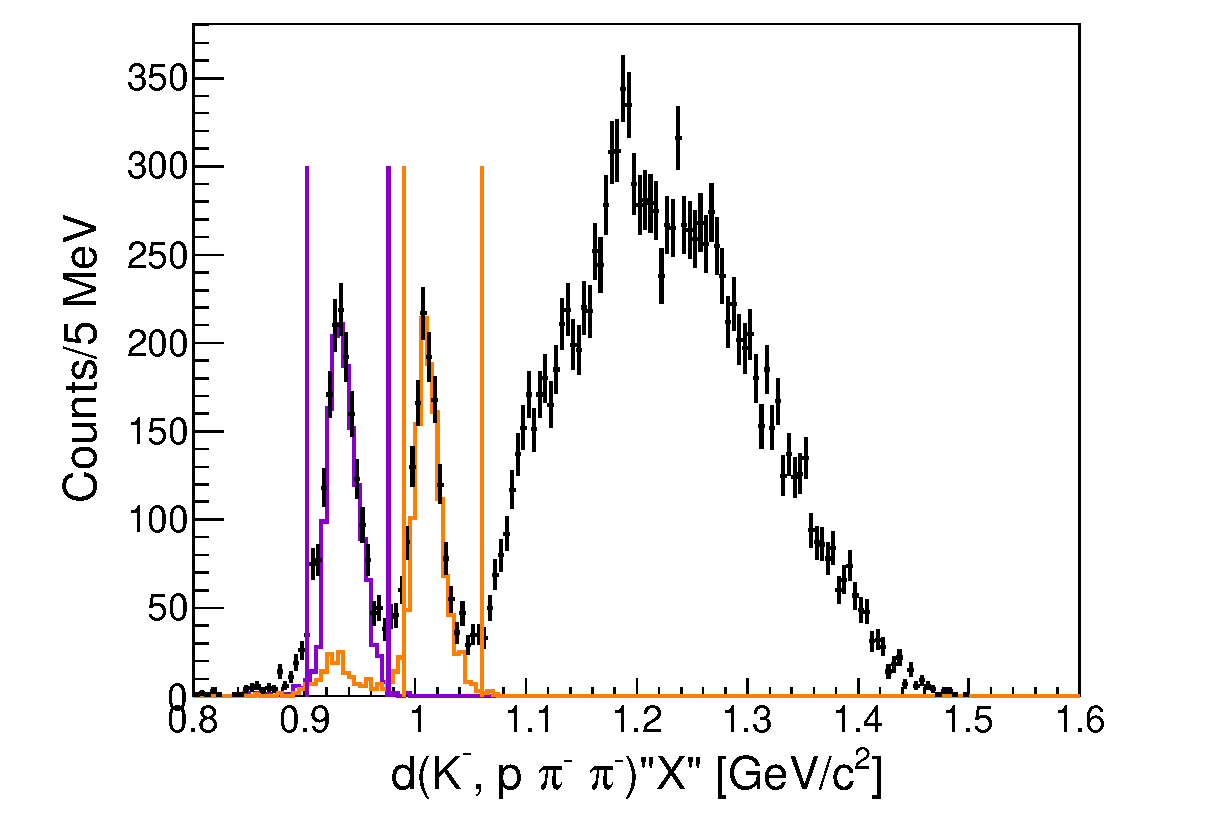
\includegraphics[width=6cm]{../pic/Run68/KP_ana/KPpimpim_MM.eps}
      \end{figure}
      \centering
      \tiny
      \vspace{-4mm}
      This figure shows $d(K^-, p \pi^- \pi^-)"X"$.
      Orange and purple plots represent $d(K^-, p \pi^-)"\Lambda"$ \& $d(K^-, p \pi^-)"\Sigma^0"$.
      Orange and purple lines shows $d(K^-, p \pi^-)"\Lambda"$ \& $d(K^-, p \pi^-)"\Sigma^0"$ selection.
      
    \end{minipage}

    \begin{minipage}{0.55\hsize}
      \begin{figure}
        \scriptsize
        No Selection\\
        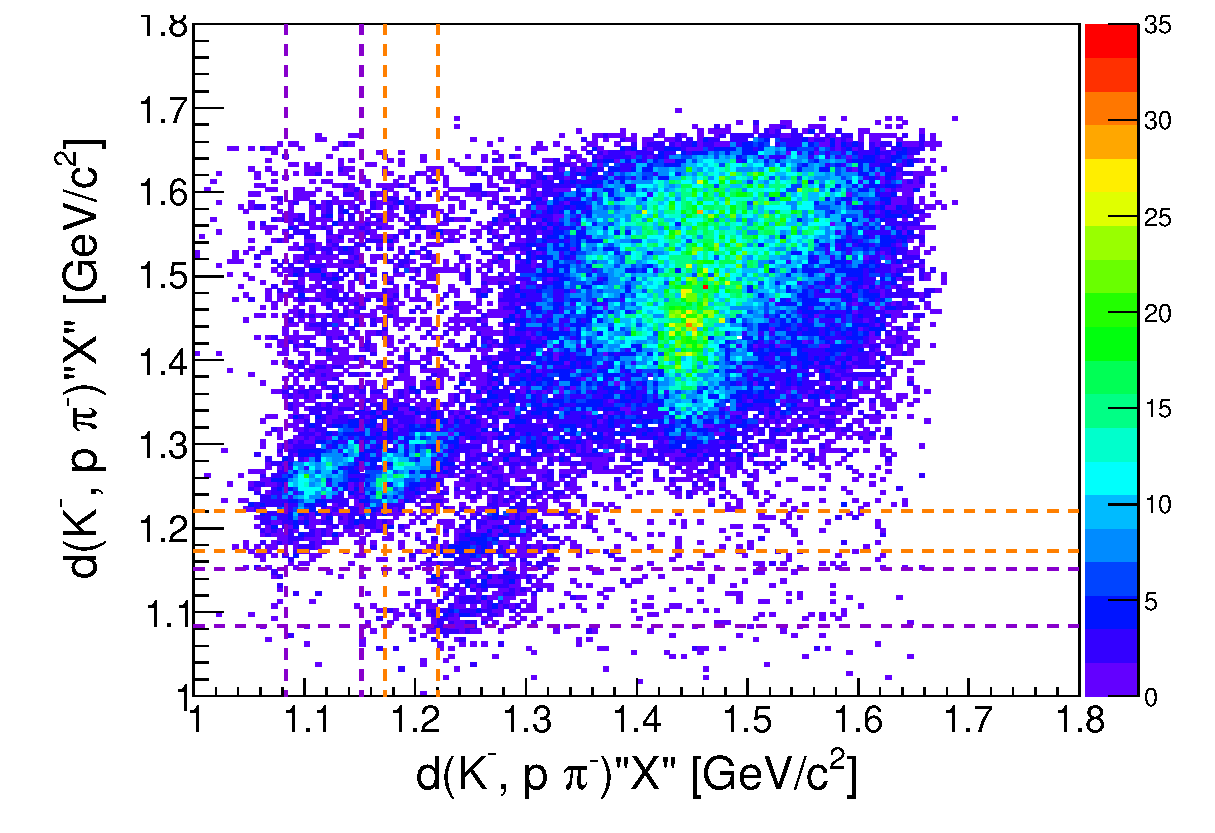
\includegraphics[width=4cm]{../pic/Run68/KP_ana/KPpim_KPpim_MM.eps}
      \end{figure}
      
      \begin{tabular}{cc}
        \begin{minipage}{0.5\hsize}
          \begin{figure}
            \scriptsize
            $d(K^-, p \pi^- \pi^-)"p"$\\ tagged\\
            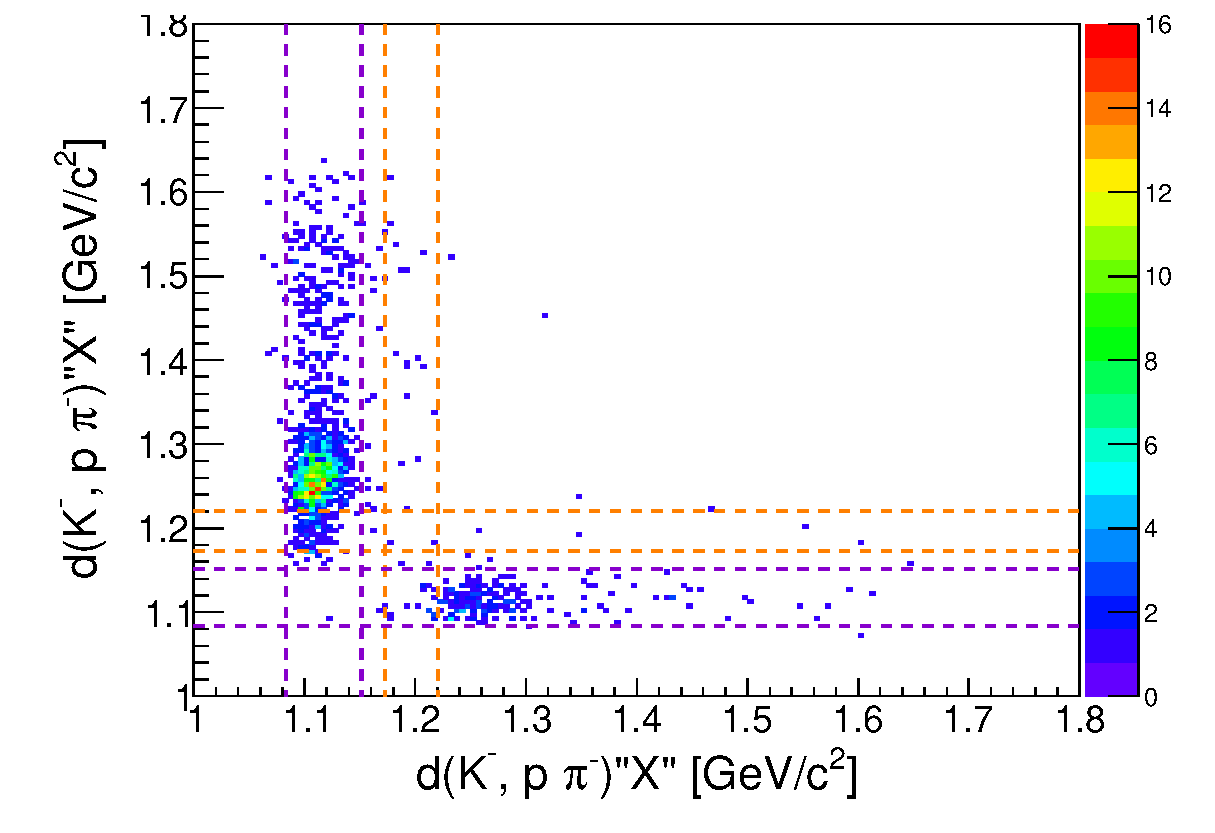
\includegraphics[width=2.5cm]{../pic/Run68/KP_ana/KPpim_KPpim_MM_mmP.eps}
          \end{figure}
        \end{minipage}

        \begin{minipage}{0.5\hsize}
          \begin{figure}
            \scriptsize
            $d(K^-, p \pi^- \pi^-)"p\gamma"$\\ tagged\\
            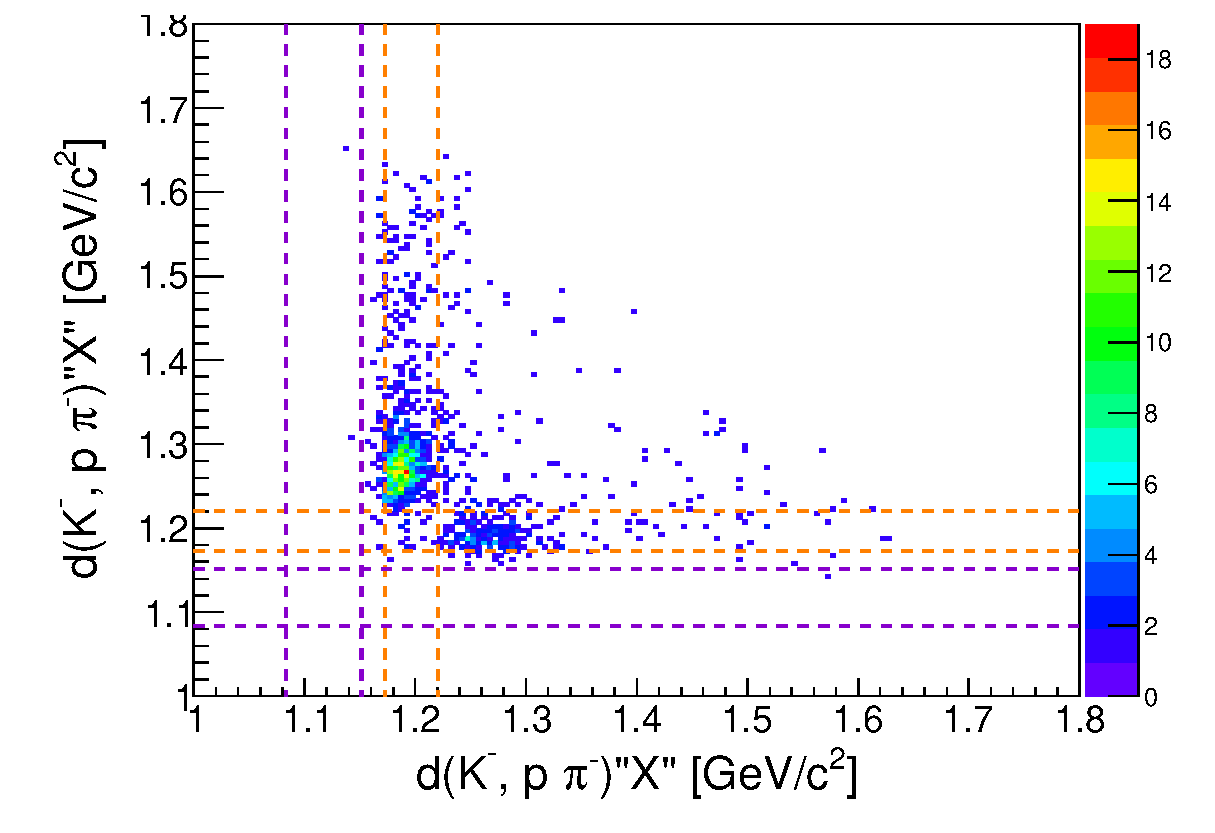
\includegraphics[width=2.5cm]{../pic/Run68/KP_ana/KPpim_KPpim_MM_mmPgamma.eps}
          \end{figure}
        \end{minipage}
      \end{tabular}
    \end{minipage}
  \end{tabular}
  \centering
  \footnotesize
  $d(K^-, p)"\pi^- \Sigma^0"$ events were selected by $d(K^-, p \pi^-)"\Sigma^0"$ \& $d(K^-, p \pi^- \pi^-)"p \gamma"$.\\
  $d(K^-, p)"\pi^- \Lambda"$ events were selected by $d(K^-, p \pi^-)"\Lambda"$ \& $d(K^-, p \pi^- \pi^-)"p"$.\\
\end{frame}
